\chapter{Installation Guide}
\label{chap:install}
After following the steps in the installation guide, TimeKeeper should be correctly installed on your system. This has been tested with Ubuntu 12.04 on both 32-bit and 64-bit systems. We are assuming you have the TimeKeeper source code.

\section{Setting up the Kernel}
\begin{itemize}
\item $cd\ /path/to/TimeKeeperSource$
\item $sudo\ ./kernel\_setup$ : This script will compile necessary scripts, download the linux-3.10.9 kernel (must have an internet connection to wget the linux kernel source) and store it in the /src directory. It will then make the necessary changes to the linux kernel.
\item Compile the newly modified kernel found at /src/linux-3.10.9. I have followed the instructions at: http://mitchtech.net/compile-linux-kernel-on-ubuntu-12-04-lts-detailed/.
\item When the modified kernel is compiled, restart the computer and load the modified kernel.
\end{itemize}

\section{Setting up CORE}
\begin{itemize}
\item $sudo\ ./core\_setup.sh$ : This script will install the necessary packages and compile CORE. You should not already have CORE installed on your system. 
\end{itemize}

\section{Setting up the TimeKeeper Kernel Module}
\begin{itemize}
\item $python\ setup\_module.py$ : The python script will ask you how many CPUs on your system you want to dedicate to TimeKeeper to use for an experiment. Then the TimeKeeper Kernel Module will be compiled. 
\end{itemize}
Congratulations! TimeKeeper is now installed.

\section{Simple Test}
With a simple test, we can see if TimeKeeper was correctly installed. 
\begin{itemize}
\item $sudo\ insmod\ ./TimeKeeper.ko$ : Insert the TimeKeeper Kernel Module into the Linux Kernel
\item $cd\ scripts$
\item $./print\_time <NumberOfLoops>$ : Run the print\_time script. This script simply does some computation, then prints out the PID, with how long it took to perform the computation in both virtual time and physical time (in format SECONDS:MICROSECONDS). This loop will be repeated NumberOfLoops. So run this for about 50 times. See figure \ref{fig:printtime} for sample print\_time output.
\item While print\_time is still running, open a new tab
\item $sudo\ ./timekeeper$-$dilate\ $-$r\ $-$p\ <pid>\ <TDF>$ : This script will dilate the process specified by PID, with a TDF specified by TDF. So use this command with the pid of the print\_time process, and a TDF of 2. 
\item Before the timekeeper-dilate command, the virtual time and physical time output of print\_time should be the same. When you dilate it, you will see the virtual time is now advancing at half the rate of physical time!
\item $sudo\ rmmod\ TimeKeeper$ : Remove the TimeKeeper Kernel Module
\end{itemize}
\begin{figure}[t]
      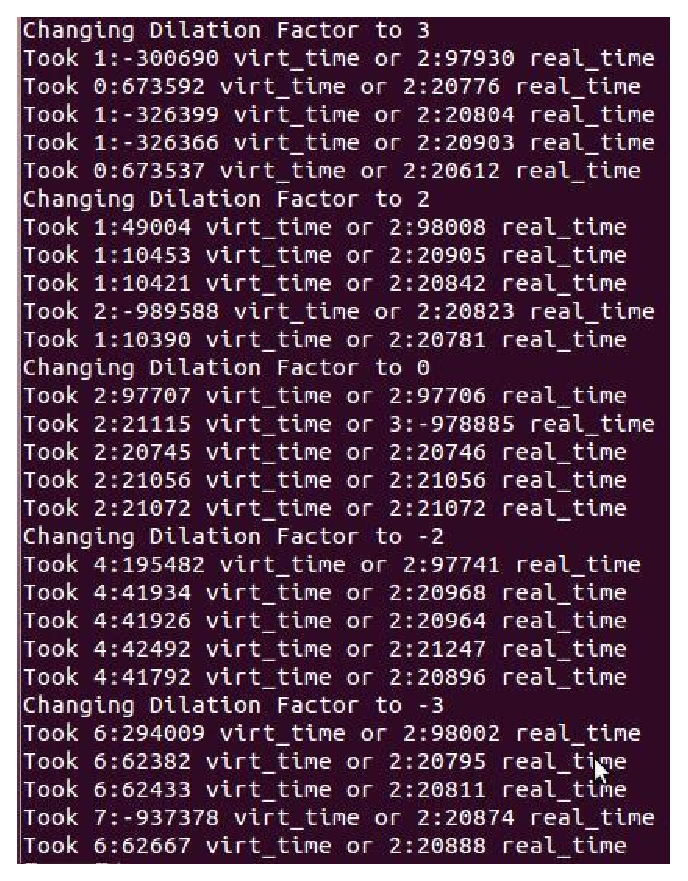
\includegraphics[width=\textwidth]{images/printtime.eps}
    \caption{Sample print\_time output }
    \label{fig:printtime}
  \end{figure}

\section{Simple CORE Experiment}
This section will explore starting a simple CORE experiment with TimeKeeper. 
\begin{itemize}
\item $sudo\ core$-$daemon\ $-$d$ : Start the CORE Daemon
\item $sudo\ insmod\ ./TimeKeeper.ko$ : Insert the TimeKeeper Kernel Module into the Linux Kernel
\item $sudo\ core$-$gui$ : Start the CORE gui. This needs to be ran as sudo to communicate with TimeKeeper
\item You should now see the CORE gui you are familiar with. You can add nodes to the GUI as you typically would. Double clicking on a host give you the ability to specify a TDF. This needs to be an integer value, see figure \ref{fig:coregui}.
\item When the topology is created, start the emulation by clicking the green 'play' button. This will create all containers, and assign them the TDFs you specified. Similar to the previous test, you may double click on a node in the gui, and run print\_time, verifying the difference between virtual time and physical time.
\item To start a synchronized experiment, navigate to the 'tools' tab, and select 'Synchronize Experiment'.
\item To stop the experiment, click on the red X
\item Remove the TimeKeeper Kernel Module when you exit out of the CORE GUI.
\end{itemize}
\begin{figure}[t]
      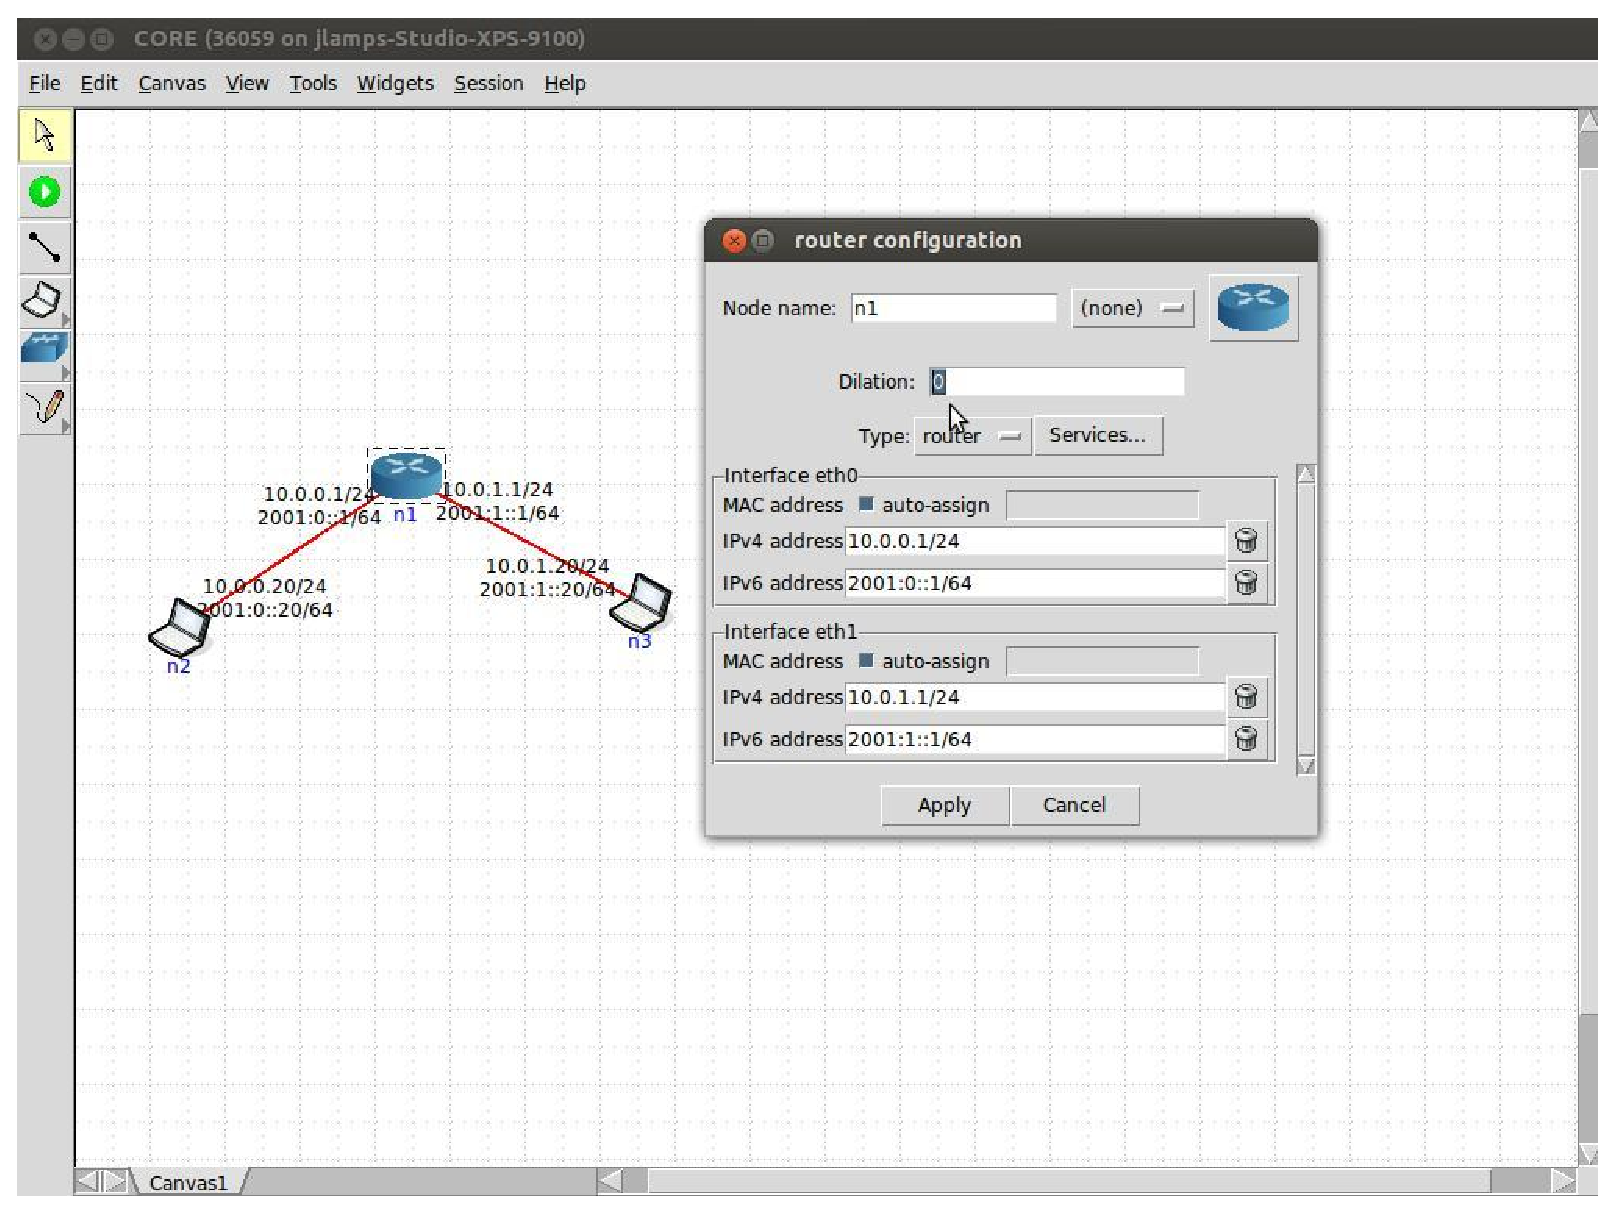
\includegraphics[width=\textwidth]{images/coregui.eps}
    \caption{CORE GUI with specifying a TDF}
    \label{fig:coregui}
  \end{figure}

\section{Simple NS-3 Experiment}
This section will describe how to start a simple ns-3 experiment with TimeKeeper with a CSMA network topology. This is assuming you already have ns-3 installed and set up on your system.
\begin{itemize}
\item $sudo\ apt$-$get\ install\ libreadline$-$dev$ : Install the necessary dependencies.
\item $cd\ /path/to/TimeKeeperSource/ns$-$3$
\item $make$ : Compile the scripts for easier LXC automation
\item $./lxcStarter\ <\#LXCs>\ <TDF>$ : When you run this command, \#LXCs will be created with the specified TDF and you will be given a prompt: 'Enter a command'.
\item Open a new terminal, and edit the file tap-csma-creator.py. Modify global variable PATH\_TO\_NS3\_TAP\_SRC and point it to the tapBridge source code within your ns-3's installation directory.
\item $python\ tap$-$csma$-$creator.py\ <\#LXCs>\ <simulatorTDF>$ : This script will create a .cc file for ns-3, with the correct number of LXCs, as well as specifying the TDF of the simulator. 
\item Move to where your ns-3 installation is, and run: $./waf\ --run\ tap$-$csma$-$virtual$-$machine$ then wait for the words TimeKeeper Integration Complete.
\item Return to the terminal where lxcStarter is running, and type $start$, this will tell TimeKeeper to start the synchronized experiment.
\item From lxcStarter, you can now send specific commands to each lxc, or all of them at once. For example, lets say you passed in the value 2 when you started lxcStarter. This will create 2 LXCs, named lxc-1 and lxc-2 with ip addresses 10.0.0.1 and 10.0.0.2 respectively. To view currently running processes within lxc-1, you would type '1 ps -A'. The first number means to send the command to lxc-1, everything after that will be what gets executed on the specified LXC. The output will be directed to /tmp/lxc-1.output. Likewise, if you want to see the files in the current directory of lxc-2, you then run '2 ls -l', and the output of the command will get written to /tmp/lxc-2.output. You can also send the same command to all LXCs at once (if you have thousands running for example) simply do '$all\ <command>$' ie: 'all ifconfig' will perform ifconfig on every LXC, and output it to /tmp/lxc-\#.output.  
\item When you are done with the experiment, send $exit$ to the lxcStarter process.
\end{itemize}

